%! TEX program = pdflatex

\documentclass[oneside,solution]{tmpl}

\usepackage[utf8]{inputenc}
\usepackage[english,ukrainian]{babel}

\title{Домашня робота}
\author{Захаров Дмитро}
\studentID{МП-31}
\instructor{Ігнатович С.Ю.}
\date{\today}
\duedate{23:59 30 квітня, 2024}
\assignno{7}
\semester{Весняний семестр 2024}
\mainproblem{Граничні цикли 2}

\begin{document}

\maketitle

% \startsolution[print]

\problem{Задача з грузиком.}

\hspace{20px}\textbf{Умова.} На конвеєрі, що рухається з постійною швидкістю $u$, стоїть вантаж масою $m$. Вантаж утримується на конвеєрі за допомогою пружини жорсткістю $k$. Нехай $x(t)$ позначає координату вантажу вздовж горизонтальної прямої (початок координат відповідає положенню вантажу, при якому пружина не стиснута і не розтягнута). На вантаж з боку конвеєра діє сила сухого тертя, яка визначається за формулою:
\begin{equation}
    F = F(\dot{x}) = \begin{cases}
        F_0, & \text{якщо} \; \dot{x} < u \\
        -F_0, & \text{якщо} \; \dot{x} > u 
    \end{cases},
\end{equation}

тобто конвеєр ``тягне за собою'' вантаж з силою, що не залежить від швидкості. При $\dot{x}=u$ вважаємо, що сила тертя не визначена. Зауважимо, що ця сила розривна.

Запишіть систему диференціальних рівнянь, побудуйте фазовий портрет та опишіть характер руху вантажу.

\textbf{Розв'язок.} Для простоти позначень, введемо коефіцієнт тертя $\mu=\frac{F_0}{mg}$. Достатньо природньо вважати $\mu \in [0,1]$ (сила тертя не може стати більше за силу тяжіння). Також, позначимо циклічну частоту $\omega^2 = \frac{k}{m}$. Отже, маємо диференціальне рівняння
\begin{equation}
    \ddot{x} +  \omega^2 x = \mu g \cdot \theta(\dot{x}), \; \theta(\dot{x}) = \begin{cases}
        1, & \dot{x} < u \\
        -1, & \dot{x} > u
\end{cases}
\end{equation}

Спочатку цікаво дослідити поведінку цієї системи, якщо в нас було б $\theta(\dot{x})=1$ завжди (це відповідає, наприклад, дуже великому значенню $u$). Тоді система набуває вигляду $\ddot{x} + \omega^2 x = \mu g$. Це рівняння можемо розв'язати явно. Зробимо заміну $z=\mu g - \omega^2 x$, тоді наше рівняння можна переписати у вигляді: $\ddot{z} + \omega^2 z = 0$. Розв'язком є $z(t) = A \cos \omega t + B \sin \omega t$, тоді наша функція $x(t)$:
\begin{equation}
    x(t) = \frac{\mu g - z(t)}{\omega^2} = \frac{\mu g}{\omega^2} + A' \cos \omega t + B' \sin \omega t
\end{equation}

По суті, цей розв'язок можна дещо спростити:
\begin{equation}
    x(t) = \frac{\mu g}{\omega^2} + x_m \cos(\omega t + \phi),
\end{equation}

де $\phi$ -- фазовий зсув. Отже, маємо звичайні гармонічні коливання, але вже навколо ненульового положення рівноваги $x_+=\frac{\mu g}{\omega^2}$. Далі будемо позначати це положення через $\ell := \frac{\mu g}{\omega^2}$.

А що станеться, якщо $\theta(\dot{x})=-1$? Наприклад, якщо конвеєр рухається з дуже великою швидкістю ліворуч? Тоді рівняння має вигляд $\ddot{x} +\omega^2 x = -\mu g$. Можна переконатись, що розв'язок цього рівняння майже аналогічний:
\begin{equation}
    x(t) = -\ell + x_m \cos (\omega t + \phi)
\end{equation}

Таким чином, знову маємо гармонічні коливання, але ненульове положення рівноваги вже $x_- = -\ell$. Таким чином, в залежності від напрямку руху конвеєра, в нас буде або положення рівноваги $-\ell$, або $+\ell$. Цей висновок буде далі корисним, проте аж ніяк не вичерпно дає відповідь на задачу, оскільки вираз $\dot{x}$ під час руху постійно то додатний, то від'ємний. 

Повернемось до початкової системи. Отже, нехай $v=\dot{x}$, тоді
\begin{equation}
    \begin{cases}
        \dot{x} = v \\
        \dot{v} = -\omega^2 x + \mu g \cdot \theta(v)
    \end{cases}
\end{equation}

Знайдемо точки спокою $(\widetilde{x},\widetilde{v})$. З першого рівняння $\widetilde{v}=0$, а з $\widetilde{x}$ ситуація така сама, як в попередньому аналізі: якщо $u>0$, то $\theta(0)=1$ і тому $\widetilde{x}=\ell$. Проте, якщо $u < 0$, то $\theta(0)=-1$ і тоді $\widetilde{x} = -\ell$. В будь-якому разі, точка спокою одна і визначається лише знаком $u$. 

Сказати тип точки дуже важко, бо ми не можемо лінеаризувати доданок $\theta(v)$. Проте далі виявиться, що перед нами центр.

Побудуємо цю систему. Цікаві два випадки: мале тертя та велике тертя. Також поки фіксуємо $u>0$, оскільки знак не принциповий для аналізу характеру руху. Результаті показані на Рисунках \ref{fig:small_friction} та \ref{fig:large_friction}.

\begin{figure}
    \centering
    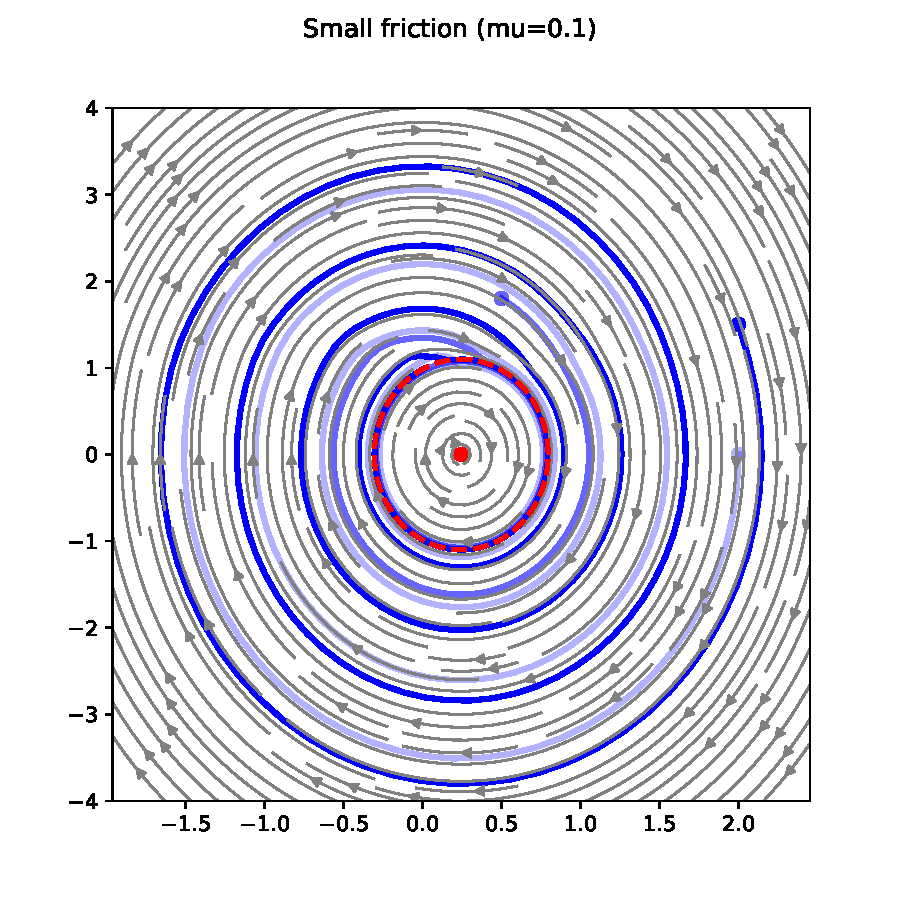
\includegraphics[width=0.65\textwidth]{images/hw_7/small_friction.pdf}
    \caption{Фазовий портрет для системи для тертя $\mu=0.1$. Інші параметри: $\omega=2 \; \text{рад}/\text{с}$, $g=9.81 \; \text{м}/\text{с}^2$, $u=1.0 \; \text{м}/\text{с}$.}
    \label{fig:small_friction}
\end{figure}
\begin{figure}
    \centering
    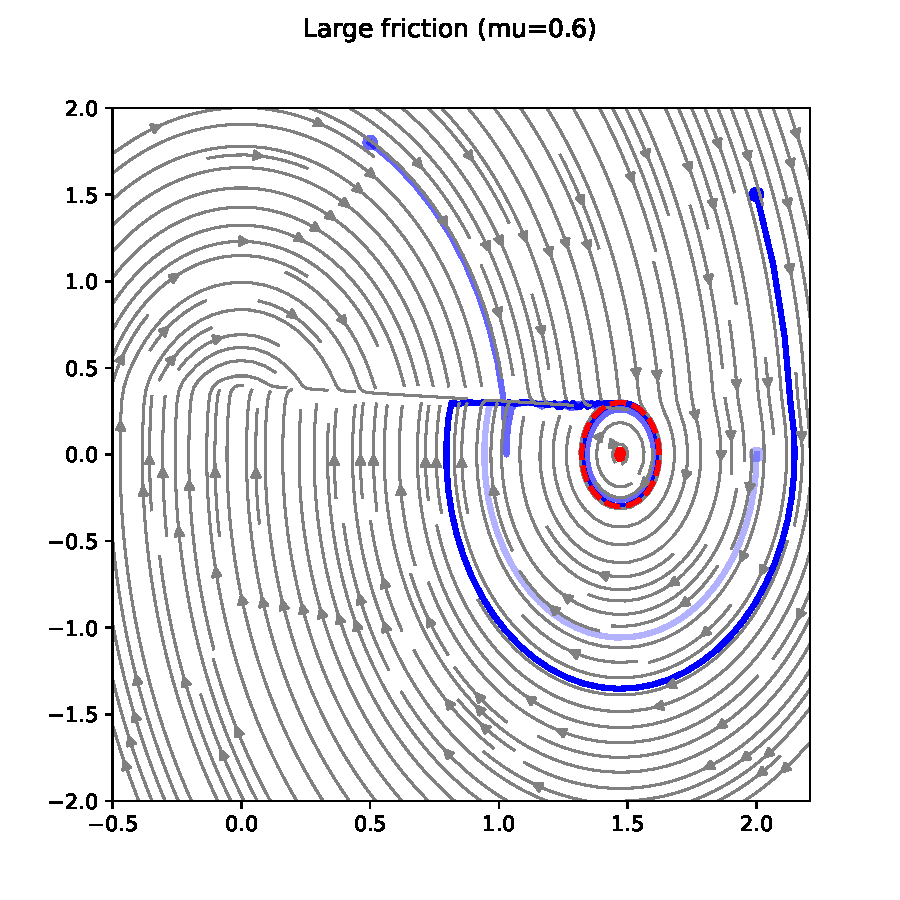
\includegraphics[width=0.65\textwidth]{images/hw_7/large_friction.pdf}
    \caption{Фазовий портрет для системи для тертя $\mu=0.7$. Інші параметри: $\omega=2 \; \text{рад}/\text{с}$, $g=9.81 \; \text{м}/\text{с}^2$, $u=0.3 \; \text{м}/\text{с}$.}
    \label{fig:large_friction}
\end{figure}

Бачимо, що рух складається з двох етапів:
\begin{itemize}
    \item Спочатку рух виглядає як затухаючі коливання.
    \item Далі рух зупиняється, якщо тертя велике -- починає рухатись з певною постійною швидкістю (далі обговоримо, з якою саме), а далі виходить на менші коливання.
\end{itemize}

Найцікавіше, що без зміни знаку тертя, не дивлячись на те, що в системі є тертя, система все одно може нескінченно рухатись (тобто наша система еквівалентна випадку без тертя, лише зі зсувом у точці рівноваги). Проте, чому тоді в нас грузик тормозить, коли є зміна знаку тертя? Річ у тому, що на фазовому портреті, коли грузик переходить пряму $v=u$, то він виходить на коло меньшого радіусу. Таким чином, після кожного перетину цієї прямої, радіус стає все меньшим і меньшим, поки швидкість не стане достатньо малою.

Цікаво також наступне -- а на яку саме швидкість виходе груз? Достатньо логічно вважати, що на швидкість конвеєра $u$. Дійсно, уявімо просту ситуацію: нехай ми відпускаємо грузик на початковій відстані $x_0>0$ з нульовою швидкістю. Звичайно, що при цьому сила тертя буде направлена праворуч, а сила пружини буде тягнути грузик ліворуч. Грузик почне рухатись лише якщо сила пружини буде більше за силу тертя: $kx_0 > \mu mg \implies x_0 > \frac{\mu mg}{k} = \ell$. В будь-якому іншому випадку, грузик не зрушиться, а отже буде просто рухатись зі швидкістю конвеєра.

Тепер нехай грузик ще і має початкову швидкість. З плином часу, швидкість коливається в певних межах від від'ємного до додатного значення, а амплітуда коливань також зменьшується. В деякий момент, швидкість стає нульовою, а координата опиняється в межах $(0,\ell)$ -- тоді грузик зупиняється і починає рухатись по прямій. 

Що відбувається далі? Оскільки грузик рухається праворуч зі швидкістю $u$, то з часом координата стає достатньо великою і грузик знову починає коливатись.

Більш того, ми можемо дуже конкретно вказати на який цикл виходить наш грузик. А саме, ми знаємо, що координата грузика при малих швидкостях описується як $x(t) = \ell + x_m\cos(\omega t+\phi)$. Оскільки грузик починає ``відриватись'' на координаті $\ell$ зі швидкістю $u$, то ця залежність набуває вигляду $x(t) = \ell + \frac{u}{\omega} \sin \omega t$. На фазову портреті, це відповідає еліпсу з півосями $u/\omega$ та $u$ з центром у $(\ell, 0)$. Він позначений червоним пунктирами на Рисунках \ref{fig:small_friction} та \ref{fig:large_friction}.

\end{document}
